\documentclass{article} % say 
\usepackage{tikz} 
\begin{document} 
We are working on 
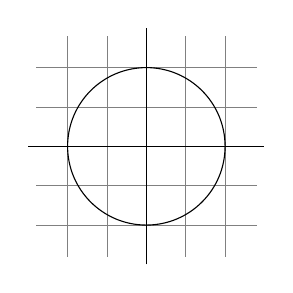
\begin{tikzpicture} 
  \draw[step=.5cm,gray,very thin] (-1.4,-1.4) grid (1.4,1.4);
  \draw (-1.5,0) -- (1.5,0); 
  \draw (0,-1.5) -- (0,1.5); 
	\draw (0,0) circle (1cm);
\end{tikzpicture}
. 
\begin{tikzpicture} 
  [Karl's grid/.style ={help lines,color=#1!50},
   Karl's grid/.default=blue]
  \draw[Karl's grid]	(0,0) grid (1.5,2);
  \draw[Karl's grid=red] (2,0) grid (3.5,2);
\end{tikzpicture}
\end{document}
